\documentclass{assignment}
\usepackage[pdftex]{graphicx} 
\usepackage{xcolor}
\definecolor{LightGray}{gray}{0.95}
%\usepackage{fancyvrb, minted} 
\usepackage[a4paper, margin = 2.5cm]{geometry} 
\usepackage[T1]{fontenc} 
% set figure path 
\graphicspath{figures}

\usepackage{amsmath, amsfonts, amssymb} 
\usepackage{hyperref, url}  
\usepackage{fancyhdr}
\usepackage{setspace}
\onehalfspacing

\student{Ahmet Akman 2442366}                             
\semester{Spring 2024}                            
\date{\today}                                   

\courselabel{EE449}          
\exercisesheet{Homework 1}{Report}  

\school{Middle East Technical University}        
\university{Electrical and Electronics Engineering}        

%%%%%%%%%%%%%%%%%%%%%%%%%%%%%%%%%%%%%%%%%%-DOCUMENT-%%%%%%%%%%%%%%%%%%%%%%%%%%%%%%%%%%%%%%%%%%%%

\begin{document}


\section{Question 1}

\subsection{Question 1.1}
\begin{figure}
    \centering
    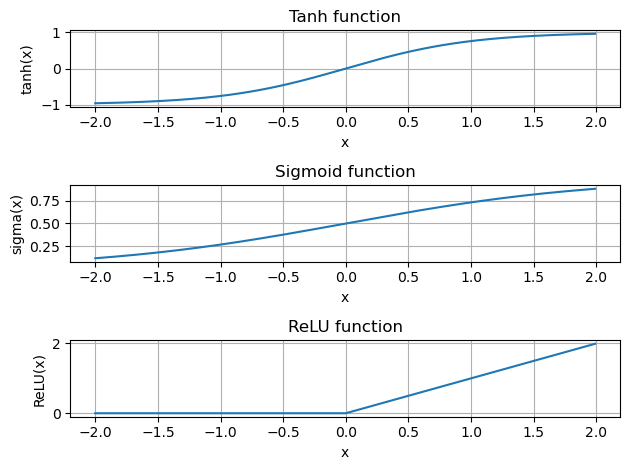
\includegraphics[width=1\textwidth]{figures/q1_1.png}
    \caption{Activation functions plot.}
    \label{fig:activation_functions}
\end{figure}



\begin{figure}
    \centering
    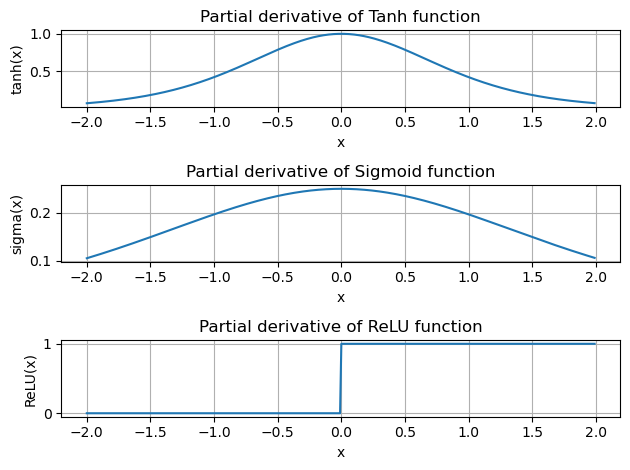
\includegraphics[width=1\textwidth]{figures/q1_2.png}
    \caption{Gradients of the activation functions plot.}
    \label{fig:activation_functions_gradient}
\end{figure}

\subsection{Question 1.2}


\begin{figure}
    \centering
    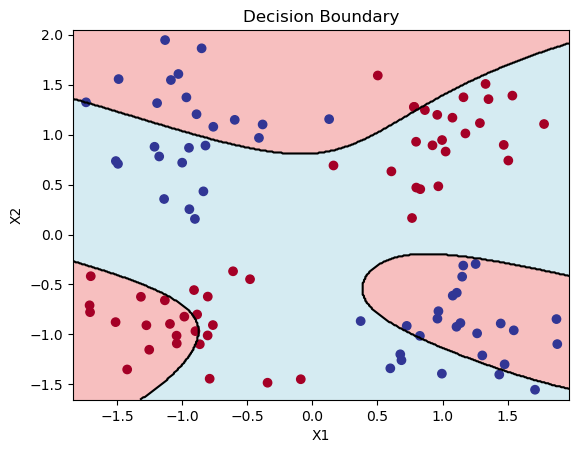
\includegraphics[width=1\textwidth]{figures/q1_sigmoid.png}
    \caption{Sigmoid activated XOR problem output.}
    \label{fig:sigmoid_q1}
\end{figure}



\begin{figure}
    \centering
    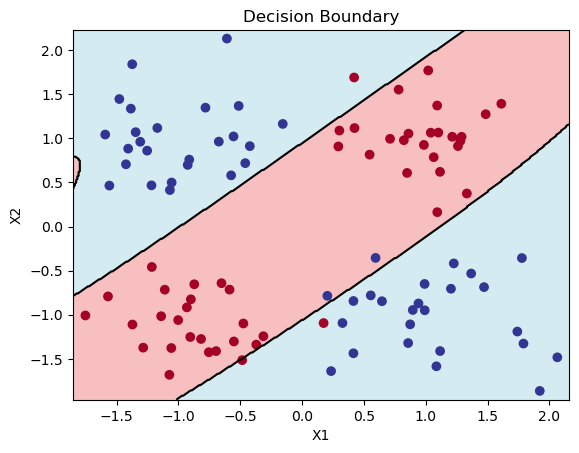
\includegraphics[width=1\textwidth]{figures/q1_tanh.png}
    \caption{Tanh activated XOR problem output.}
    \label{fig:tanh_q1}
\end{figure}

\begin{figure}
    \centering
    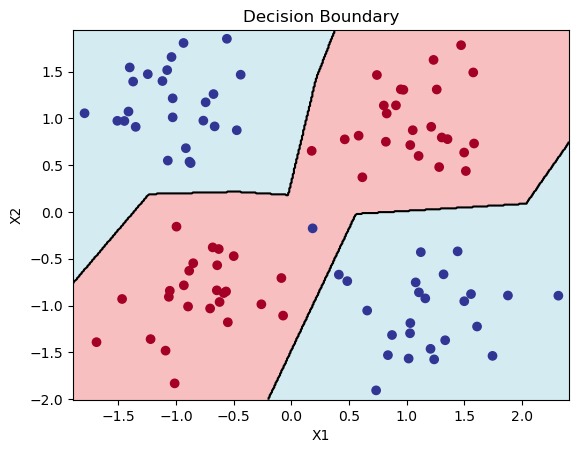
\includegraphics[width=1\textwidth]{figures/q1_relu.png}
    \caption{ReLU activated XOR problem output.}
    \label{fig:relu_q1}
\end{figure}
\section{Question 2}

\section{Question 3}

\section{Question 4}

\section{Question 5}



%--------------------------------------BIBLIOGRAFIA-------------------------------------------

\newpage
\section{References}
\nocite{*} 
\bibliographystyle{ieeetr}   
\bibliography{refs}     


\end{document}